\documentclass[a4paper,12pt]{article}

	\usepackage[utf8]{inputenc}
	\usepackage[T1]{fontenc}
	
	\usepackage[notes=true]{lib/dtrt}
	\usepackage{algorithm}
	\usepackage{algpseudocode}
	\usepackage{amsmath}
	\usepackage{xcolor}
	\usepackage{graphicx}
	\usepackage{todonotes}
	\usepackage{listings}
	\usepackage{pxfonts}
	\usepackage[margin=1in]{geometry}

	\usepackage{lib/lang}  % include language definition for protobuf
	\usepackage{lib/style} % include custom style for proto declarations.	
	
	%\usepackage{sagetex}

	\makeatletter
	\newcommand{\subparhead}[1]{\smallskip \noindent {\itshape\ignorespaces \dt@MaybeAddPunct{#1}}\hskip 0.9em plus 0.3em minus 0.3em \dt@ignorespacesandimplicitepars}
	\makeatother

	% Auuthor notes (using dtrt's macros). Switch the dtrt package flag to notes=false to hide.
	\definecolor{darkgreen}{rgb}{0,0.6,0}
	\newcommand{\dnote}[1]{\dtcolornote[Daniel]{red}{#1}}
	\newcommand{\anote}[1]{\dtcolornote[Aurell]{blue}{#1}}
	\newcommand{\enote}[1]{\dtcolornote[Eran]{darkgreen}{#1}}

	\newcommand\dtodo[1]{\todo[color=red!20]{#1}}
	\newcommand\atodo[1]{\todo[color=green!20]{#1}}
	\newcommand\etodo[1]{\todo[color=blue!20]{#1}}
	\def\boxit#1{%
		\smash{\color{red}\fboxrule=1pt\relax\fboxsep=-2pt\llap{\rlap{\fbox{\strut\makebox[#1]{}}}~}}\ignorespaces
	}

	% Style for identifiers.
	\newcommand{\textid}[1]{\texttt{#1}}
	% Note paragraphs.
	\newcommand{\noteparagraph}[1]{\textbf{#1}.}
	
	%\makeatletter
	%\def\BState{\State\hskip-\ALG@thistlm}
	%\makeatother
	
	%opening
	\title{zkInterface, a standard tool for zero-knowledge interoperability}
	\author{Daniel Benarroch, Kobi Gurkan, Aurélien Nicolas, Eran Tromer}
	
	\begin{document}
		
		\maketitle
		 
% \enote{Add abstract}
\tableofcontents
%=============================================================================
\section{Overview}
This standard, part of the ZKProof Standardization effort \cite{ZKProofSecurity, ZKProofImplementation, ZKProofApplications}, aims to facilitate interoperability between ZK proof implementations, at the level of the low-constraint systems that are produced by frontends (and represent application-level statements) and consumed by cryptographic backends. The high-level goal is to enable decoupling of frontends from backends, allowing application writers to choose the frontend most convenient for their functional and development needs and combine it with the backend that best matches their performance and security needs. This includes communicating constraint systems, communicating variable assignments (for production of proofs), and also construction of constraint systems out of smaller building blocks (gadgets) possibly implemented by different authors and frameworks.

This first revision focuses on non-interactive proof systems (NIZKs) for general statements (i.e., NP relations) represented in the R1CS/QAP-style constraint system representation\footnote{R1CS (i.e., a set of bilinear constraints where linear combinations are ``for free'' is the native language of the numerous ZK schemes based on Quadratic Arithmetic Programs, which are used by most deployment nowadays. Moreover, arithmetic circuits and Boolean circuits can be easily and efficiently reduced to R1CS. Hence the focus on R1CS in this initial revision.}. This includes many, though not all, of the practical general-purpose ZKP schemes currently deployed. While this focus allows us to define concrete formats for interoperability, we recognize that additional constraint system representation styles (e.g., arithmetic and Boolean circuits and algebraic constraints) are in use, and are within scope of future revisions.
%\enote{Add reference to R1CS. I think the best one, in term of notations and references, we have is the QED-it challenge... We prepared a PDF stand-alone version of that for ZKProof, maybe post it online or attach it as an appendix?}

An implementation of the zkInterface \cite{zkinterface} can be found in the following GitHub repository \href{https://github.com/QED-it/gadget_standard}{QED-it/gadget\_standard}.
%-----------------------------------------------------------------------------
\subsection{Background}

Zero-Knowledge Proofs are cryptographic primitives that allow some entity (the prover) to prove to another party (the verifier) the validity of some statement or relation. Today there are many efficient constructions of NIZKs, each with different trade-offs, as well as several implementations of the proving systems. By standardizing zero-knowledge proofs, we aim to foster the proper use of the technology.

Every proving system can be divided \cite{ZKProofImplementation} into the backend, which is the portion of the software that contains the implementation of the underlying cryptographic protocol, and the frontend, which provides means to express statements in a convenient language, allowing to prove such statements in zero knowledge by compiling them into a low-level representation of the statement.

The backend of a proving system consists of the key generation, proving and verification algorithms. It proves statements where the instance and witness are expressed as variable assignments, and relations are expressed via low-level languages (such as arithmetic circuits, Boolean circuits, R1CS/QAP constraint systems or arithmetic constraint satisfaction problems). There are numerous such backends, including implementations of many of the schemes discussed in the Security Track proceeding \cite{ZKProofSecurity}.

The frontend consists of the following:
\begin{itemize}
	\item The specification of a high-level language for expressing statements.
	\item A compiler that converts relations expressed in the high-level language into the low-level relations suitable for some backend(s). For example, this may produce an R1CS constraint system.
	\item Instance reduction: conversion of the instance in a high-level statement to a low-level instance (e.g., assignment to R1CS instance variables).
	\item Witness reduction: conversion of the witness to a high-level statement to a low-level witness (e.g., assignment to witness variables).
	\item Typically, a library of "gadgets" consisting of useful and hand-optimized building blocks for statements.
\end{itemize}

Since the offerings and features of backends and frontends evolve rapidly, we refer the reader to the curated taxonomy at \url{https://zkp.science} for the latest information.  

Currently, existing frontend are implemented to work best with their corresponding backend, the proving system is usually built end-to-end. The frontend compiles a statement into the native representation used by the cryptographic protocol in the backend, in many cases without explicitly exposing the constraint system compilation to the user. Moreover, if the compilers can output intermediary files and configurations, they are usually in a non-standard format. In practice this means that
\begin{itemize}
	\item There is no portability between different backends and frontends, and
	\item It is not possible to generate a constraint system using different frontends
\end{itemize}   

With this proposal we aim to solve this by creating a R1CS-based interface between frontends and backends, as seen in Figure \ref{interface}. We add an explicit formatting layer between the frontends and backends that allows the user to ``pick-and-chose'' which existing frontend and backend they prefer. Furthermore, given the programatic design of our interface, a specific component, or gadget, can itself call a sub-component from a different frontend. This enables the use of more than one frontend to generate the complete statement.

\begin{figure}[h!]
	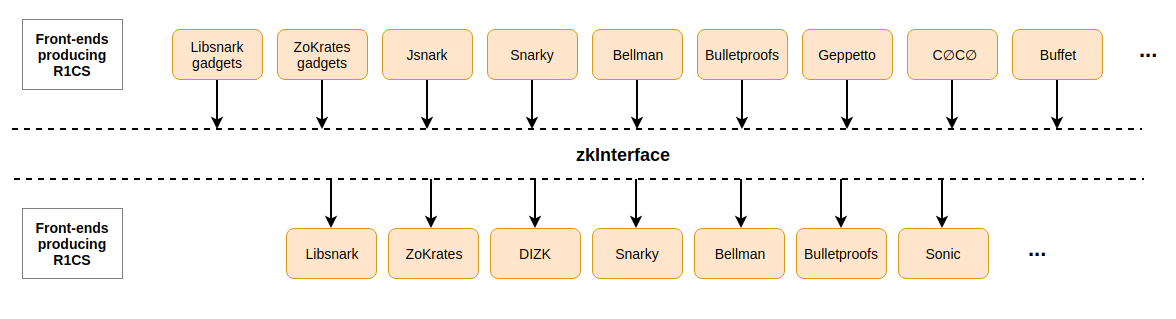
\includegraphics[width=\linewidth]{graphics/interop.png}
	\caption{Interoperability between frontends and backends with zkInterface}
	\label{interface}
\end{figure}

%-----------------------------------------------------------------------------
\subsection{Terminology}
The terminology follows the Implementation Track proceeding \cite{ZKProofImplementation}, and any new terms and concepts will be defined accordingly.

\subsection{Goals} 
\label{goals}

There are several forms of interoperability and we set some of these as goals for this standard. One such form is between different implementations of the same backend construction, providing an interoperable format for the proving and verification keys, as well as the proof. Another form is between backends and frontends, which is the focus of this standard. The following are stronger forms of the latter kind of interoperability which have been identified as desirable by practitioners.

\parhead{Statement instance and witness formats} 
Specifying a standard format for the statement instance and witness enables users to have their choice of frameworks (frontends and backends) and streaming for storage and communication, and facilitate creation of benchmark test cases that could be executed by any backend accepting these formats.
 
Crucially, analogous formats are desired for constraint system languages other than R1CS.

\parhead{Statement semantics, variable representation and mapping}

Beyond the above, there’s a need for different implementations to coordinate the semantics of the statement (instance) representation of constraint systems. For example, a high-level protocol may have an RSA signature as part of the statement, leaving ambiguity on how big integers modulo a constant are represented as a sequence of variables over a smaller field, and at what indices these variables are placed in the actual R1CS instance.

Precise specification of statement semantics, in terms of higher-level abstraction, is needed for interoperability of constraint systems that are invoked by several different implementations of the instance reduction (from high-level statement to the actual input required by the ZKP prover and verifier). One may go further and try to reuse the actual implementation of the instance reduction, taking a high-level and possibly domain-specific representation of values (e.g., big  integers) and converting it into low-level variables. This raises questions of language and platform incompatibility, as well as proper modularization and packaging.

Note that correct statement semantics is crucial for security. Two implementations that use the same high-level protocol, same constraint system and compatible backends may still fail to correctly interoperate if their instance reductions are incompatible -- both in completeness (proofs don’t verify) or soundness (causing false but convincing proofs, implying a security vulnerability). Moreover, semantics are a requisite for verification and helpful for debugging. Beyond interoperability, some low-level building blocks (e.g., finite field and elliptic curve arithmetic) are needed by many or all implementations, and suitable libraries can be reused.

Some backends can exploit uniformity or regularity in the constraint system (e.g., repeating patterns or algebraic structure), and could thus take advantage of formats and semantics that convey the requisite information.

Given the typical complexity level of today’s constraint systems, it is often acceptable to handle all of the above manually, by fresh re-implementation based on informal specifications and inspection of prior implementation. Our goal, however, is for the interface to handle the semantics of the components, reducing the predisposition to error as application complexity grows. The following paragraphs expand on how the semantics should be considered for interoperability of gadgets.

\parhead{Witness reduction}
Similar considerations arise for the witness reduction, mapping a high-level witness representation for a given statement into the assignment to witness variables (as defined by the instance). For example, a high-level protocol may use Merkle trees of particular depth with a particular hash function, and a high-level instance may include a Merkle authentication path. The witness reduction would need to convert these into witness variables, that contain all of the Merkle authentication path data encoded by some particular convention into field elements and assigned in some particular order. Moreover, it would also need to convert the numerous additional witness variables that occur in the constraints that evaluate the hash function, ensure consistency and Booleanity, amonh others.

\parhead{Gadgets interoperability}
Beyond using fixed, monolithic constraint systems and their assignments, there is a need for sharing subcircuits and gadgets. For example, libsnark offers a rich library of R1CS gadgets, which developers of several front-end compilers would like to reuse in the context of their own constraint-system construction framework. 

While porting chunks of constraints across frameworks is relatively straightforward, there are challenges in coordinating the semantics of the externally-visible variables of the gadget, analogous to but more difficult than those mentioned above for full constraint systems. Mainly, there is a need to coordinate or reuse the semantics of a gadget’s externally-visible variables (those accessible by other gadgets), as well as the witness reduction function of imported gadgets in order to assign a witness into the internal variables of the gadget.

As for instance semantics, well-defined gadget semantics is crucial for soundness, completeness and verification, and is helpful for debugging.

\parhead{Procedural interoperability}
An attractive approach to the aforementioned needs for instance and witness reductions (both at the level of whole constraint systems and at the gadget level) is to enable one implementation to invoke the instance/witness reductions of another, even across frameworks and programming languages.

This requires communication not of mere data, but invocation of procedural code. Suggested approaches to this include linking against executable code (e.g., .so files or .dll), using some elegant and portable high-level language with its associated portable, or using a low-level portable executable format such as WebAssembly. All of these require suitable calling conventions (e.g., how are field elements represented?), usage guidelines and examples.


\subsection{Desiderata}
The following requirements that guide our design, within the large space of possibilities for achieving the above goals.

\begin{enumerate}
	\item Interoperability across frontend frameworks and programming languages.
	\item Ability to write components that can be consumed by different frontends and backends.
	\item Minimize copying and duplication of data.
	\item The overhead of the R1CS construction and witness reduction should be low (and in particular, linear) compared to a native implementation of the same gadgets in existing frameworks.
	\item Expose details of the backend's interface that are necessary for performance (e.g., constraint system representation and algebraic fields).
	\item The approach can be extended to support constraint systems beyond R1CS.
\end{enumerate}

\subsection{Scope, limitations and possible extensions}

We present a set of specifications to be standardized to enable the use of an interface between zero-knowledge proof systems. We have identified the minimal items needed to create a standard interface that meets the goals and desired requirements. The following points form the scope of our proposed standard.

\begin{itemize}
	\item Standard defined messages that the caller and callee exchange.
	\item The serialization of the messages.
	\item A protocol to build a constraint system from gadget composition.
	\item Technical recommendations for implementation.
\end{itemize}

Some limitations of the standard, with respect to interoperability, are the following.

\parhead{Limitations.}
The following are not addressed by this standard:

\subparhead{Backend interoperability} We do not aim to standardize the proof algorithms, the format of the proofs generated by a backend, or the format of the proving and verification keys -- all of which would be required to achieve interoperability between backends. (See ``Proof interoperability'' and ``Common reference strings'' in \cite{ZKProofImplementation}.

\subparhead{Programming language and frontend frameworks} We are intentionally agnostic about, and do not aim to standardize, the programming language and programming framework used by frontends.

\parhead{Extensions.}
The following are not covered by the present revision of the standard, but should be covered by future extensions. Thus, the standard should be flexible enough and easy to extend in a backward-compatible compatible fashion, to achieve the following:

\subparhead{Other constraint system representations.}
Going beyond R1CS, we plan on supporting other constraint system representations that are native to some ZK backends. These include Boolean circuits, arithmetic circuits, and algebraic constraint systems.

\subparhead{Uniform constraint systems}
Some backends can take advantage of uniformity in the constraint system (e.g., when some elements are repeated many times). Support the expression of such uniformity in the constraint system representation, so backends can take utilize it.

\subparhead{Packaging} Describe self-contained packaging of a component would allow for portable execution of the components (or gadgets) on different platforms.

\subparhead{Typing} Enforcing properties of variables using a type system (e.g., a ``boolean variable'' type that ensures a variable is 0 or 1 even when working over a large field).

%=============================================================================
\section{Design}
\label{sec:design}

%-----------------------------------------------------------------------------
\subsection{Approach}

	zkInterface is a procedural, purely functional interface for zero-knowledge systems that enables cross-language interoperability. The current version, even if limiting, creates an interface based on R1CS formatting and offers the ability to abstractly craft a constraint system building from different gadgets, possibly written in different frameworks, by defining how data should be written and read.
	It is independent of any particular proving systems.

	The same interface can be used in two use-cases:
	\begin{itemize}
		\item To connect the construction and execution of a zero-knowledge program
			to a proving system. See Figure \ref{fig:programproving}.

		\item To decompose a zero-knowledge program into multiple gadgets that can be engineered separately. See Figure \ref{fig:programcomponents}.
	\end{itemize}
	
\begin{figure}[!h]
	\centering
	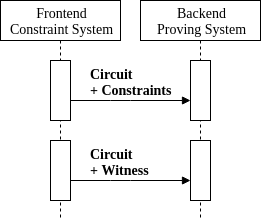
\includegraphics[width=0.5\linewidth]{graphics/program_proving.png}
	\caption{The interaction between a zero-knowledge program and a proving system.}
	\label{fig:programproving}
\end{figure}

\begin{figure}[!h]
	\centering
	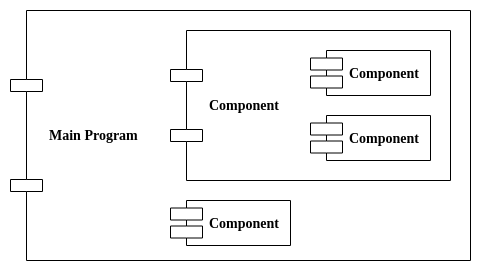
\includegraphics[width=0.7\linewidth]{graphics/program_components.png}
	\caption{A zero-knowledge program built from multiple gadgets.}
	\label{fig:programcomponents}
\end{figure}


\parhead{Interface}

	The interaction between caller and gadgets is based on exchanging messages.
	Messages are purely read-only data, which grants a great flexibility to
	implementations of gadgets and applications.

\parhead{Interoperability}

	Different parts of an application may be written in different programming languages, and interoperate through messages.
	These parts may be linked and executed in a single process, calling functions,
	and exchanging messages through buffers of shared memory.
	They may also run as separate processes, writing and reading messages in files, or through pipes or sockets.
	Some implementation strategies are discussed in section~\ref{sec:implementation}.

\parhead{Messages Definition \label{messagedefinition}}

	The set of messages is defined in Listing \ref{zkinterface.fbs},
	using the FlatBuffers interface definition language.
	All messages and fields are defined in this schema.

	The FlatBuffers system includes an interface definition language
	which implies a precise data layout at the byte level.
	Code to write and read messages can be generated for all common programming languages.
	Examples are provided for C++ and for Rust.

	Multiple paths for evolution and extensions of the standard are possible,
	thanks to the flexibility and backward-compatibility features of the encoding.
	The encoding is designed to require little to no data transformation, making it possible
	to implement the standard with minimal overhead in very large applications.

	Messages must be prefixed by the size of the message not including the prefix,
	as a 4-bytes little-endian unsigned integer.
	This makes it possible to concatenate and distinguish messages
	in streams of bytes or in files.

	The specification of FlatBuffers can be found at
	\href{https://google.github.io/flatbuffers/}{https://google.github.io/flatbuffers/}.


\parhead{Instance and Witness Reductions}

	Instance reduction is the process of constructing a constraint system.
	Witness reduction is the process of assigning values to all variables
	in the system before generating a proof about concrete input values.

	When using a proving system with pre-processing, instance reduction
	is performed once ahead of time and used in a trusted setup.
	In proving systems without pre-processing, instance reduction is used in proof verification.
	The standard supports both execution flows.


%-----------------------------------------------------------------------------
\subsection{Architecture}

\begin{figure}[!h]
	\centering
	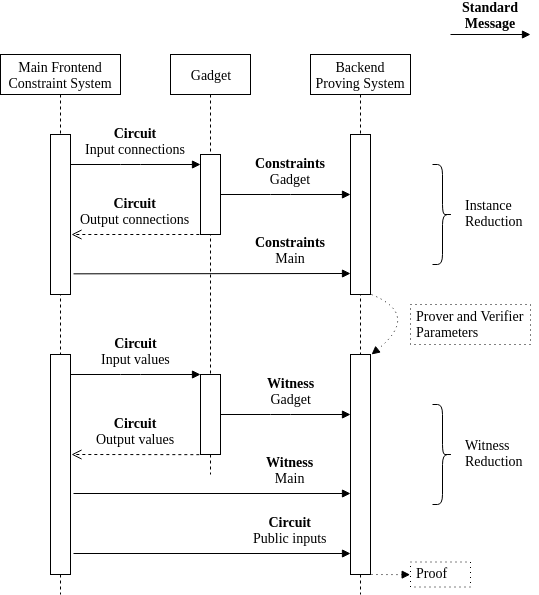
\includegraphics[width=\linewidth]{graphics/call_flow.png}
	\caption{The flow of messages between libraries using the interface.}
	\label{fig:flow}
\end{figure}

\parhead{Messages Flow}
	The flow of messages is illustrated in Figure \ref{fig:flow}.

	The caller calls the gadget code with a single \textid{GadgetCall} message.
	The gadget exits with a single \textid{GadgetReturn} message.
	This is a control flow analoguous to a function call in common programming languages.

	The caller can request an instance reduction, or a witness reduction, or both at once.
	This is controlled by the fields \textid{generate\_r1cs} and \textid{generate\_assignment} of \textid{GadgetCall} messages.

	During instance reduction,
	a gadget may add any number of constraints to the constraint system
	by sending one or more \textid{R1CSConstraints} messages.
	The caller and other gadgets may do so as well.

	During witness reduction,
	a gadget may assign values to variables
	by sending one or more \textid{AssignedVariables} messages.

\parhead{Messages Channels}
	The caller provides the gadget with the means to send messages,
	or output channels.	This can be implemented in various ways depending
	on the application.
	The caller may arrange a distinct channel for each message type,
	and the gadget must send messages to the appropriate channels.

	\noteparagraph{Note}
	This design allows a gadget to call other gadgets itself.
	All \textid{R1CSConstraints} or \textid{AssignedVariables} messages
	from all (sub-)gadgets may be sent to a shared channel
	without the need to aggregate them into a single message,
	and independently of the call/return flow.
	Moreover, an implementation can decouple the proving system
	from the logic of building constraints and assignments,
	by arranging for the constraints and assignments messages
	to be processed by the proving system, independently from the control logic.

\parhead{Variables}
	The constraint system reasons about variables, which are assigned a numerical identifier that are unique within a constraint system. The variable numbers are incrementally allocated in a global namespace. Messages that contain constraints or assignments refer to variables by this numeric ID. It is up to gadgets that create the constrain system to keep track of the semantics (and if desired, helpful symbolic names) of the variables that they deal with, and to allocate new variables for their internal use. The messages defined by the framework include a simple protocol for conveying the state of of the variable allocator (i.e., the first free variable number), and the identity of variables that tie a gadget to other gadgets.

	\noteparagraph{Note}
	This design allows implementations to aggregate and handle messages in a generic way,
	without any	reference to the gadgets or mechanisms that generated them.

\parhead{Local Variables Allocation}
	A gadget may allocate a number of local variables to use
	in the internal implementation of the function that it computes.
	They are analoguous to stack variables in common programming languages.

	The following protocol is used to allocate variable IDs that are
	unique within a whole constraint system.
	\begin{itemize}
		\item The caller must provide a numerical ID greater than all IDs that have already been allocated, called the Free-Before ID.
		\item The gadget may use the Free-Before ID and consecutive IDs as its local variables IDs.
		\item The gadget must return the next consecutive ID that it did not use, called the Free-After ID.
		\item The caller must treat IDs lesser than the Free-After ID as allocated by the gadget,
			and must not use them.
	\end{itemize}

	During instance reduction, the gadget can refer to
	its local variables in the\\
	\textid{R1CSConstraints} messages that it generates.
	The caller and other parts of the program must not refer to these local variables.

	During witness reduction, the gadget must assign values to its local variables
	by sending \textid{AssignedVariables} messages.

\parhead{Incoming/Outgoing Variables}

	The concept of incoming, outgoing variables arises when a program is decomposed into gadgets.
	These variables serve as the functional interface between a gadget and its caller.
	They are analoguous to arguments and return values of functions in common programming languages.
	A variable is not inherently incoming, outgoing, nor local;
	rather, this is a convention in the context of a gadget call.

	The caller provides the IDs of variables to be used as incoming and outgoing variables by the gadget.
	There may be no outgoing variables if the gadget implements a pure assertion.

	During instance reduction, both the caller and the gadget can refer to
	these variables in the \textid{R1CSConstraints} messages that they generate.
	Other parts of the program may also refer to these same variables in their own contexts.

	During witness reduction, the caller must pass incoming values to the gadget in the \textid{GadgetCall} message.
	The gadget must return outgoing values to the caller in the \textid{GadgetReturn} message.

	The caller is responsible for the assignment of values to both incoming and outgoing variables.
	How this is achieved depends on the caller and proving system,
	and on whether some variables are treated as public inputs of the instance.



\subsection{Interface Definition}

A copy of the messages definition is hosted at \\
\href{https://github.com/QED-it/gadget_standard/blob/master/zkinterface.fbs}{https://github.com/QED-it/gadget\_standard/blob/master/zkinterface.fbs}

\lstinputlisting[
	caption=Messages Definition,
	language=flatbuffers2,style=protobuf,
	label=zkinterface.fbs]{../zkinterface.fbs}


%=============================================================================
\section{Implementation}
\label{sec:implementation}

The above section describes a protocol and the format of messages.
Applications can execute, and exchange messages with
gadgets and proving systems implementations in a variety of ways.
We recommend two approaches in this section.

\parhead{In-memory execution}
\label{inmemory}

The application may execute the code of a component in its own process.

The component exposes its functionnality as a function calleable using the C calling convention of the platform. The component code may be linked statically or be loaded from a shared library.

The application must prepare a ComponentCall message in memory, and implement one callback functions to receive the messages of the component,
and call the component function with pointers to the message and the callbacks.

The component function reads the call message and performs its specific computation. It prepares the resulting messages (of type R1CSConstraints, AssignedVariables, or GadgetReturn) in memory, and calls the callbacks with pointers to these messages.

A function definition that implements this flow is defined in Listing \ref{gadget.h} as a C header. Refer to the inline documentation for more details.


\parhead{Multi-process execution}

Different parts of the application can be implemented as different
programs, executed separately.

As specified in section~\ref{message_definition}, messages are framed and typed,
and can be concatenated in a stream of bytes. It is therefore possible to connect multiple programs through UNIX-style pipes, or to arrange a program to write messages to a file for another program to read later.
To process multiple messages from the same stream or file, a program
reads the 4 bytes containing the size of the next message, allowing it to seek
to the message after that.

A program that constructs a constraint system or implements a gadget should read a GadgetCall message from the standard input stream (stdin).
It should write one or more messages of type R1CSConstraints or AssignedVariables to the standard output stream (stdout).
It should write a single GadgetReturn message to the standard error stream
(stderr, used as a control channel).

A program that implements a proving system should read messages of type R1CSConstraints, AssignedVariables, or GadgetReturn from stdin,
which should contain all the information needed to perform a pre-processing
or to generate proofs.


\parhead{Demonstration}

An example implementation is provided.

A number of C++ helper functions are used to interoperate
with libsnark protoboard objects.
A SHA256 gadget from libsnark/gadgetlib1
is encapsulated with the message-based interface of section~\ref{sec:design}.

A test program written in Rust demonstrates
in-memory execution using the method in section~\ref{inmemory},
and includes helper functions to process messages.

This code can be found at \href{https://github.com/QED-it/gadget\_standard}{https://github.com/QED-it/gadget\_standard}.


\lstinputlisting[
	caption=zkinterface.h - C Interface,
	language=C++,style=protobuf,
	label=zkinterface.h]{../cpp/zkinterface.h}


\begin{thebibliography}{99}
	\bibitem{ZKProofSecurity}
	1st ZKProof Standards Workshop,
	\emph{Security Track Proceeding}.
	Online at \href{https://zkproof.org}{ZKProof.org}.
	Published in Cambridge, Massachusetts, on May, 2018.

	\bibitem{ZKProofImplementation}
	1st ZKProof Standards Workshop,
	\emph{Implementation Track Proceeding}.
	Online at \href{https://zkproof.org}{ZKProof.org}.
	Published in Cambridge, Massachusetts, on May, 2018.

	\bibitem{ZKProofApplications}
	1st ZKProof Standards Workshop,
	\emph{Applications Track Proceeding}.
	Online at \href{https://zkproof.org}{ZKProof.org}.
	Published in Cambridge, Massachusetts, on May, 2018.

	\bibitem{zkinterface}
	D. Benarroch, K. Gurkan, A. Nicolas, E. Tromer, \emph{gadget\_standard: an implementation of zkInterface}.
	Online at \href{https://github.com/QED-it/gadget_standard}{github.com/QED-it/gadget\_standard}.
	Tel Aviv, Israel, 2019.
\end{thebibliography}
 
 
\end{document}